% 一年级上册 第一单元综合训练(重做版)
% 原卷是横向的两页对开(第 89、90 页),这里改成两张竖向 A4,单面打印即可。
% 编译:xelatex 试卷.tex
\documentclass[a4paper,12pt,fontset=mac]{ctexart}
\usepackage[top=12mm,bottom=10mm,left=16mm,right=16mm]{geometry}
\usepackage{tikz}
\usetikzlibrary{shapes.geometric}
\usepackage{xeCJK}
\pagestyle{empty}
\setlength{\parindent}{0pt}
\linespread{1.15}

\newcommand{\sect}[2]{\vspace{4mm}{\heiti\bfseries\large #1}\;{\small #2}\par\vspace{2mm}}
\newcommand{\blank}{(\hspace{9mm})}
\newcommand{\bx}{\tikz[baseline=-0.6ex]\draw (0,0) rectangle (7.5mm,7.5mm);}
\newcommand{\bxs}{\tikz[baseline=-0.6ex]\draw (0,0) rectangle (6mm,6mm);}
\newcommand{\cir}{\tikz[baseline=-0.6ex]\draw (0,0) circle (3.6mm);}

% 一个盘子,\plate{桃子数}。桃子位置按堆叠摆好(0~5 个)
\newcommand{\plate}[1]{%
\begin{tikzpicture}[baseline=0]
  \draw[thick] (0,0) ellipse (13mm and 3mm);
  \draw (0,0) ellipse (10mm and 2mm);
  \ifcase#1
  \or \fill[orange!70] (0,2.5mm) circle (2.6mm);
  \or \fill[orange!70] (-3mm,2.5mm) circle (2.6mm); \fill[orange!70] (3mm,2.5mm) circle (2.6mm);
  \or \foreach \x/\y in {-5/2.2,0/2.2,5/2.2} {\fill[orange!70] (\x mm,\y mm) circle (2.6mm);}
  \or \foreach \x/\y in {-5/2.2,0/2.2,5/2.2} {\fill[orange!70] (\x mm,\y mm) circle (2.6mm);}
      \fill[orange!70] (0,6.5mm) circle (2.6mm);
  \or \foreach \x/\y in {-7/2.2,-2.5/2.2,2.5/2.2,7/2.2} {\fill[orange!70] (\x mm,\y mm) circle (2.6mm);}
      \fill[orange!70] (0,6.5mm) circle (2.6mm);
  \fi
  \ifnum#1>0 \foreach \x/\y in {0/0} {} \fi
\end{tikzpicture}}

% 数字格:\strip{a,b,c,...} 空串表示要填的格子
\newcommand{\strip}[1]{%
\begin{tikzpicture}[baseline=-1mm]
  \foreach \t [count=\i from 0] in {#1} {
    \draw (\i*9mm,0) rectangle ++(9mm,9mm);
    \node at (\i*9mm+4.5mm,4.5mm) {\t};
  }
\end{tikzpicture}}

% 对比两列图形:\cmp{左个数}{右个数}{左形状}{右形状}
\tikzset{
  sa/.style={star,star points=5,fill=black!70,inner sep=0pt,minimum size=5.5mm},
  sb/.style={diamond,fill=black!35,inner sep=0pt,minimum size=5.5mm,aspect=0.9},
  sc/.style={circle,fill=orange!70,draw,inner sep=0pt,minimum size=5mm},
  sd/.style={regular polygon,regular polygon sides=3,fill=green!50!black!70,inner sep=0pt,minimum size=5.5mm},
  se/.style={rectangle,fill=blue!45,inner sep=0pt,minimum size=4.5mm},
  sf/.style={ellipse,fill=yellow!70!orange,draw,inner sep=0pt,minimum width=7mm,minimum height=4mm},
}
\newcommand{\cmp}[4]{%
\begin{tikzpicture}[baseline=-24mm]
  \useasboundingbox (-3mm,3.5mm) rectangle (25mm,-24mm);
  \foreach \i in {1,...,#1} {\node[#3] at (0,-\i*7mm+7mm) {};}
  \foreach \i in {1,...,#2} {\node[#4] at (22mm,-\i*7mm+7mm) {};}
  \pgfmathtruncatemacro{\m}{min(#1,#2)}
  \foreach \i in {1,...,\m} {\node at (11mm,-\i*7mm+7mm) {$\cdots$};}
\end{tikzpicture}}

% 数的分解树:\tree{上}{左}{右},空串画方框
\newcommand{\nn}[1]{\ifx&#1&\bxs\else\makebox[6mm]{#1}\fi}
\newcommand{\tree}[3]{%
\begin{tikzpicture}[baseline=0]
  \node (t) at (0,10mm) {\nn{#1}};
  \node (l) at (-8mm,0) {\nn{#2}};
  \node (r) at (8mm,0) {\nn{#3}};
  \draw (t.south) -- ++(0,-1.5mm) -- (l.north);
  \draw (t.south) -- ++(0,-1.5mm) -- (r.north);
\end{tikzpicture}}

% 一串珠子:白黑交替,共 9 颗
\newcommand{\beads}{%
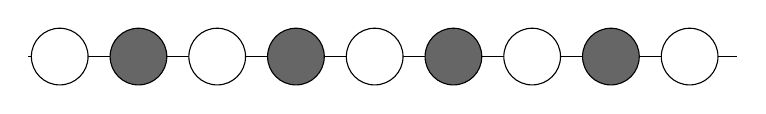
\begin{tikzpicture}[baseline=-0.6ex]
  \draw (-4mm,0) -- (86mm,0);
  \foreach \i in {0,...,8} {
    \pgfmathparse{mod(\i,2)==0?"white":"black!60"}
    \edef\c{\pgfmathresult}
    \draw[fill=\c] (\i*10mm,0) circle (3.6mm);
  }
\end{tikzpicture}}

% 一个袋子,\bag{饼干数}
\newcommand{\bag}[1]{%
\begin{tikzpicture}[baseline=0]
  \draw[thick] (0,0) .. controls (-9mm,0) and (-9mm,11mm) .. (-2mm,15mm)
     -- (2mm,15mm) .. controls (9mm,11mm) and (9mm,0) .. (0,0);
  \draw[thick] (-3mm,15mm) -- (3mm,15mm) -- (4mm,18mm) -- (-4mm,18mm) -- cycle;
  \ifcase#1
  \or \draw[fill=yellow!50] (0,6mm) circle (2.3mm);
  \or \draw[fill=yellow!50] (-2.8mm,6mm) circle (2.3mm); \draw[fill=yellow!50] (2.8mm,6mm) circle (2.3mm);
  \or \draw[fill=yellow!50] (-3mm,4mm) circle (2.3mm); \draw[fill=yellow!50] (3mm,4mm) circle (2.3mm);
      \draw[fill=yellow!50] (0,8.5mm) circle (2.3mm);
  \or \draw[fill=yellow!50] (-3mm,3.5mm) circle (2.3mm); \draw[fill=yellow!50] (3mm,3.5mm) circle (2.3mm);
      \draw[fill=yellow!50] (-3mm,8.5mm) circle (2.3mm); \draw[fill=yellow!50] (3mm,8.5mm) circle (2.3mm);
  \or \draw[fill=yellow!50] (-3mm,3.5mm) circle (2.3mm); \draw[fill=yellow!50] (3mm,3.5mm) circle (2.3mm);
      \draw[fill=yellow!50] (-3mm,8.5mm) circle (2.3mm); \draw[fill=yellow!50] (3mm,8.5mm) circle (2.3mm);
      \draw[fill=yellow!50] (0,6mm) circle (2.3mm);
  \fi
\end{tikzpicture}}

\begin{document}

%================= 第 1 页(原第 89 页) =================
\begin{center}
  {\heiti\bfseries\fontsize{20}{26}\selectfont 第一单元综合训练}\\[2mm]
  {\small 训练时间:60 分钟\qquad 满分:100 分+10 分}
\end{center}
\vspace{1mm}
姓名:\underline{\hspace{35mm}}\qquad 日期:\underline{\hspace{35mm}}\qquad 得分:\underline{\hspace{25mm}}
\vspace{2mm}

\begin{center}{\heiti\bfseries\large 知识技能}\;{\small (78 分)}\end{center}

\sect{一、我会填。}{(每空 1 分,共 32 分)}

{\bfseries 1.}根据盘子中的桃子数量写数。\par\vspace{3mm}
\hspace{-1mm}%
\begin{tabular}{@{}c@{\hspace{5mm}}c@{\hspace{5mm}}c@{\hspace{5mm}}c@{\hspace{5mm}}c@{}}
\plate{3} & \plate{4} & \plate{1} & \plate{0} & \plate{5}\\[2mm]
\bx & \bx & \bx & \bx & \bx
\end{tabular}

\vspace{3mm}
{\bfseries 2.}按顺序填数。\par\vspace{2mm}
\hspace{4mm}\strip{,1,2,3,,}\hspace{12mm}\strip{5,,3,2,,}

\vspace{3mm}
{\bfseries 3.}一个对一个连一连,再在方框里填数、在 $\bigcirc$ 里比大小。\par\vspace{2mm}
\hspace{4mm}%
\begin{tabular}{@{}c@{\hspace{14mm}}c@{\hspace{14mm}}c@{}}
\cmp{4}{2}{sa}{sb} & \cmp{3}{4}{sc}{sd} & \cmp{4}{4}{se}{sf}\\[2mm]
\bx\ {\Large $>$}\ \bx & \bx\ {\Large $<$}\ \bx & \bx\ {\Large $=$}\ \bx
\end{tabular}

\vspace{3mm}
{\bfseries 4.}填一填(分与合)。\par\vspace{3mm}
\hspace{4mm}%
\tree{}{2}{2}\hspace{10mm}\tree{5}{}{3}\hspace{10mm}\tree{}{2}{1}\hspace{10mm}\tree{5}{1}{}\hspace{10mm}\tree{2}{}{}

\vspace{3mm}
{\bfseries 5.}\quad\beads\quad{\small $\bigcirc$ 有\blank 个,\ $\bullet$ 有\blank 个,}\par\vspace{2mm}
\hspace{4mm}$\bigcirc$ 比 $\bullet$\blank (填“多”或“少”)1 个。

\vspace{2mm}
{\bfseries 6.}看图填一填。\par\vspace{2mm}
\begin{center}
\begin{tabular}{@{}c@{\hspace{14mm}}c@{\hspace{14mm}}c@{\hspace{14mm}}c@{\hspace{14mm}}c@{}}
\bag{3} & \bag{5} & \bag{1} & \bag{4} & \bag{2}
\end{tabular}
\end{center}
\vspace{1mm}
\hspace{4mm}(1)\ 从左边数,第 1 袋有\blank 块饼干。\par\vspace{1mm}
\hspace{4mm}(2)\ 从左边数,有 5 块饼干的是第\blank 袋。\par\vspace{1mm}
\hspace{4mm}(3)\ 从右边数,有 1 块饼干的是第\blank 袋。\par\vspace{1mm}
\hspace{4mm}(4)\ 从左边数,第\blank 袋和第\blank 袋合起来有 3 块饼干。

\vfill
\centerline{\small 数学\ --\ 89\ --\ 一年级·上册}
\newpage

%================= 第 2 页(原第 90 页) =================
\sect{二、我会算。}{(共 28 分)}

{\bfseries 1.}直接写出得数。(12 分)\par\vspace{7mm}
\begin{tabular}{@{}p{40mm}p{40mm}p{40mm}p{40mm}@{}}
$3-1=$ & $5-1=$ & $2+3=$ & $1+2=$\\[15mm]
$3+0=$ & $0+5=$ & $4+1=$ & $4-4=$\\[15mm]
$0+0=$ & $5-3=$ & $4-2=$ & $2+2=$
\end{tabular}

\vspace{13mm}
{\bfseries 2.}在 $\bigcirc$ 里填上“$>$”“$<$”或“$=$”。(8 分)\par\vspace{7mm}
\begin{tabular}{@{}p{40mm}p{40mm}p{40mm}p{40mm}@{}}
$4+1\ \cir\ 5$ & $0+4\ \cir\ 3$ & $4-3\ \cir\ 2$ & $5-1\ \cir\ 4$\\[15mm]
$3\ \cir\ 3-1$ & $0\ \cir\ 4-0$ & $4\ \cir\ 2+2$ & $3-3\ \cir\ 3$
\end{tabular}

\vspace{13mm}
{\bfseries 3.}在 $\bigcirc$ 里填上“$+$”或“$-$”,使等式成立。(8 分)\par\vspace{7mm}
\begin{tabular}{@{}p{40mm}p{40mm}p{40mm}p{40mm}@{}}
$2\ \cir\ 2=4$ & $5\ \cir\ 3=2$ & $4\ \cir\ 1=5$ & $5\ \cir\ 2=3$\\[15mm]
$4\ \cir\ 1=3$ & $2\ \cir\ 3=5$ & $3\ \cir\ 2=1$ & $5\ \cir\ 4=1$
\end{tabular}

\vspace{13mm}
\sect{三、我会选。}{(将正确答案的序号填在括号里)(10 分)}

{\bfseries 1.}与 $4-2$ 的得数相等的加法算式是(\hspace{8mm})。\par\vspace{4mm}
\hspace{10mm}\textcircled{\small 1}\ $0+1$\hspace{22mm}\textcircled{\small 2}\ $3-1$\hspace{22mm}\textcircled{\small 3}\ $1+1$

\vfill
\centerline{\small 数学\ --\ 90\ --\ 一年级·上册}

\end{document}
